\documentclass{tufte-handout}
%\usepackage{tikz}
\usepackage{booktabs}
\usepackage{siunitx}
\usepackage{adjustbox}
\usepackage{graphicx}

%following 3 packages + new command are for sexy listings (code representation):
\usepackage{listings}
\usepackage[most]{tcolorbox}
\usepackage{inconsolata}
\newtcblisting[auto counter]{sexylisting}[2][]{sharp corners, fonttitle=\bfseries, colframe=gray, listing only, listing options={basicstyle=\ttfamily\footnotesize, language=java,breaklines=true}, title=Source \thetcbcounter: #2, #1} 


\title{Word Ladders}
\author{by Group Z\\ Lucas Beck, Eva Bertels, Kristin Kaltenh\"{a}user, Sune T\o nder}

\begin{document}
\maketitle

\section{Word Ladders Report}

\section{Results}
% NOT EDITED YET
  Our implementation called \texttt{MyDigraph} produces the expected results on all input--output file pairs, 
  On input {\tt words-5757.txt}, a shortest path from prawn to bread of length/distance four is the following:
  \begin{quotation}
     prawn -> warns -> nears ->  saber -> bread 
  \end{quotation}

  \section{Implementation details}

  We build the graph's edges by iterating over all words in the word-xxx.txt file and loading them into a symbol table.
  The value of each word represents its index in \texttt{adj}.
  
  To build the graph, we take the last four characters of each word and compare it to all other words in the symbol table.
  \texttt{matchVertices()} creates an array of characters for the complete word.
  If one of the four characters we are looking for is present in this array, it is deleted, so that same letters are not counted twice.
  If all four letters are present in the array without repetition, the index of this word is added to the \texttt{adj} of the first word.  
  
  The running time for graph construction is $O(n^2)$,
  as we have to iterate through all n vertices and find    their edges for both directions.
    
    
   
  To measure the length of the path, we create a breadth-first-search (bfs) for the vertex corresponding to the first word with the \texttt{BreadthFirstDirectedPath} file provided by the book and calling the method \texttt{distTo}.
 We receive the path calling another method, namely\texttt{bfs.pathTo}.

% ADD RUNNING TIME AND REMOVE SIDENOTE:
  The total running time of our implementation (including graph construction and doing a traversal for 1 word pair) is 
$n^2 * w + n + m$  
where n is edges, m is vertices, and w is the length of the word.

Because of the slow build time, our wordladder was not able to run the final file \texttt{word-in-104500.txt} within a reasonable amount of time.
But if given enough processing power and time, it was able to complete. Its output, can be seen in the following picture(To save you the time needed to run this).


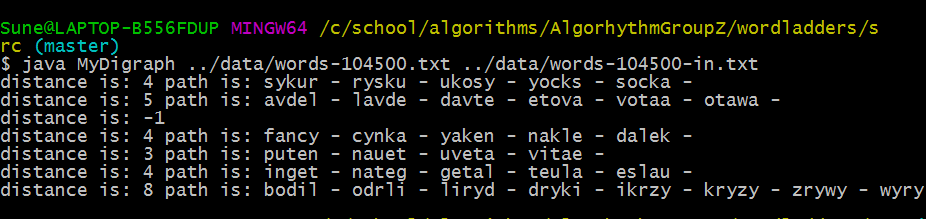
\includegraphics{largefile.png}


\end{document}